%%%%%%%%%%%%%%%%%%%%%%%%%%%%%%%%%%%%%%%%%%%%%%%%%%%%%%%%%%%%%%%%%%%%%%%%%%%%%%%%
% reconstruction.tex:
%%%%%%%%%%%%%%%%%%%%%%%%%%%%%%%%%%%%%%%%%%%%%%%%%%%%%%%%%%%%%%%%%%%%%%%%%%%%%%%%
\chapter{Event Reconstruction}
\label{sec:reco_chapter}
%%%%%%%%%%%%%%%%%%%%%%%%%%%%%%%%%%%%%%%%%%%%%%%%%%%%%%%%%%%%%%%%%%%%%%%%%%%%%%%%

Electrons, muons and jets expected from \WR and \nul decays traversed multiple CMS sub-detectors, 
as shown in Figure \ref{fig:particleTrajectories}.  Their trajectories and energies were measured 
from charged particle tracks reconstructed by the silicon tracker, and energy deposits reconstructed 
by the calorimeters and the muon detectors.  The high energy of expected leptons and jets motivated 
the use of specific lepton and jet reconstruction algorithms described herein.

\begin{figure}[h]
	\centering
	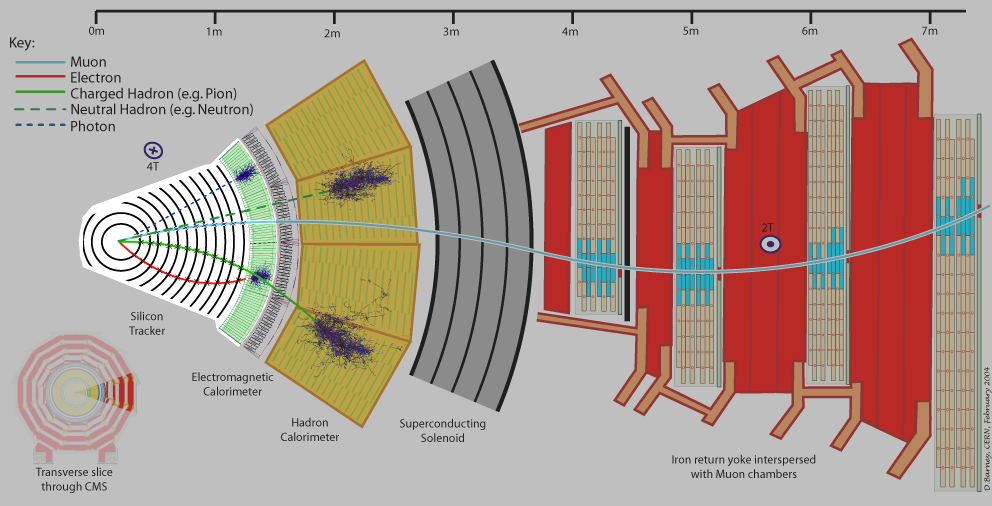
\includegraphics[width=0.75\textwidth]{figures/flowOfParticlesThroughCMS.png}
	\caption{Typical trajectories of particles travelling through CMS, from CERN.}
	\label{fig:particleTrajectories}
\end{figure}


\section{Muon Reconstruction}
\label{sec:muReco}
Muons were first reconstructed as tracks from hits in the silicon tracker.  An interative algorithm started 
by reconstructing tracks from the highest energy hits and hits closest to the IP, and progressed to outer layers 
using a Kalman filter to link hits between successive layers.  Once the algorithm reached the outermost tracker 
layer the hits associated with tracks were removed from the list of track candidates, and a new track 
reconstruction iteration started with hits in the innermost pixel layers that had lower energy or were further 
from the IP.  It was assumed that the magnetic field was uniform, and tracks were reconstructed as perfect helixes 
from hits in consecutive layers.  If two or more tracks shared a common origin point, that point was reconstructed 
as an interaction vertex, whose position was measured relative to the IP.  Isolated muons with 
$\pt > 0.9$ $\GeV$ and $|\eta| < 2.4$ were reconstructed with essentially 100\% efficiency \cite{trackerPerformanceInCollisions}.  
Muons with $|\eta| < 1.4$ and $\pt = 100$ $\GeV$ and their vertices were measured with resolutions of approximately 
2.8\% in $\pt$, and 10 and 30 $\mu$m in transverse and longitudinal distances from the IP.  Muon trajectories and 
initial energies were determined by tracker measurements, and their energies were refined by muon detector measurements.

After traversing the calorimeters and the magnet, muons were reconstructed as tracks from hits in muon detector chambers.  
First, local reconstruction was run to build track segments in individual chambers, then an iterative track 
reconstruction algorithm built continuous tracks from multiple segments.  The muon track reconstruction algorithm started 
with track segments in the inner muon chambers, then iterated outward and built longer tracks across multiple chambers 
using a Kalman filter.  The algorithm estimated the effects of energy losses, inhomogenous magnetic fields, and multiple 
scattering when linking segments between chambers, and updated all track parameters after including measurements 
from each new chamber.  Once the algorithm incorporated measurements from the outermost chambers, a Kalman filter 
was applied to the reconstructed tracks, starting with the outermost chamber segments and working towards the 
innermost chamber segments, to ensure the tracks were built in a self-consistent way \cite{muonRecoFirstCollisions}.  

Muons were reconstructed and their momenta were determined using silicon tracker and muon detector measurements.  
Tracks reconstructed in the muon detectors were extrapolated back to the outermost silicon tracker layer, and in the 
plane of the silicon strip each reconstructed muon was identified as a muon detector track that matched a silicon 
tracker track to within 3 cm.  After reconstruction, the $\pt$ of each muon was calculated using the following procedure.  
Four muon reconstruction algorithms fitted four continuous tracks \cite{cmsMuonRecoRunTwo} to silicon tracker and muon 
detector hits to estimate a muon's trajectory through CMS, as represented in Figure \ref{fig:particleTrajectories}.  Each 
algorithm combined muon detector and silicon tracker measurements in a different way, and could exclude measurements with 
large uncertainty.  The quality of each continuous track was identified by a fit uncertainty $\chi^{2}/nDOF$ and momentum 
uncertainty $\sigma(\pt)/\pt$.  The track with the lowest uncertainties was used to calculate the reconstructed muon 
momentum.  For muons with $\pt \lesssim 100$ $\GeV$ this procedure used tracker measurements almost exclusively to 
determine the muon momentum; as stated earlier, muons with $|\eta| < 1.4$ and $\pt = 100$ $\GeV$ were measured with a 
$\pt$ resolution of approximately 2.8\%.  As the muon $\pt$ increased above 100 $\GeV$ the silicon tracker $\pt$ 
resolution degraded faster than the muon detector $\pt$ resolution, and it became advantageous to combine measurements 
from both detectors.  Muons with $\pt > 200$ $\GeV$ were expected in a significant fraction of $\WR \rightarrow \mu\mu jj$ 
events (Table \ref{tab:wrHighPtMuons}), and for $|\eta| < 0.9$ and $200 < \pt < 400$ $\GeV$ they were measured with a 
$\pt$ resolution of 3.2\%; for $\pt > 400$ $\GeV$ the resolution was better than 6\% \cite{cmsMuonRecoRunTwo}.

\begin{table}[h]
	\caption{Fraction of expected $\WR \rightarrow \mu\mu jj$ events that had at least one muon with $\pt > 200$ $\GeV$. 
	($\mnul = \frac{1}{2}\mWR$)}
	\label{tab:wrHighPtMuons}
	\centering
	\begin{tabular}{c|c}
		\mWR ($\TeV$) & Fraction of events with at least one high-$\pt$ muon (\%) \\  \hline
		1.0 &  80.  \\
		2.0 &  95.  \\ 
		3.0 &  98.  \\ \hline
	\end{tabular}
\end{table}

Following momentum calculations, the momenta of muons were corrected using $Z \rightarrow \mu\mu$ decays.  $Z \rightarrow \mu\mu$ 
events in data and simulations were compared, and two differences were found.  The dilepton mass distribution in simulated 
events was narrower, indicating better energy resolution, and the peak (in $\GeV$) was higher, indicating a higher 
energy scale.  Both the energy resolution and scale affect the efficiency of muon $\pt$ requirements, so the 
$\pt$ of muons in data and simulated events were corrected such that the $Z \rightarrow \mu\mu$ dilepton mass peak 
positions and widths were identical.


\section{Electron Reconstruction}
\label{sec:eleReco}
Electrons ($e^{\pm}$) were the only particles from \WR decays expected to lose more than a few percent of their 
energy before reaching the ECAL.  One to two radiation lengths of material, depending on $\eta$, was in front of 
the ECAL \cite{ecalPerformanceInCollisions}, and about 35\% of electrons lose more than 70\% of their initial energy 
through bremsstrahlung before reaching the ECAL \cite{trackerPerformanceInCollisions}.  The curvature of electrons 
in the magnetic field meant that bremsstrahlung photons emitted by the electrons, in general, struck the ECAL 
at $\eta$ values similar to that of the electron, but at different $\phi$ coordinates.  The tracker could not detect 
these photons, but knowledge of electron bremsstrahlung was incorporated into a dedicated electron track reconstruction 
algorithm.  The fractional energy lost by electrons traversing a tracker layer through bremsstrahlung was expected to 
have a distribution described by the Bethe-Heitler formula, and this energy loss was approximated as a sum of 
several Gaussians in the electron track reconstruction algorithm.  The electron algorithm was otherwise identical to 
the muon track reconstruction algorithm, except that the $\chi^{2}$ threshold used to 
associate tracker hits with a trajectory was loosened from 30 to 2000 \cite{trackerPerformanceInCollisions}.  This 
facilitated the reconstruction of electron tracks whose trajectories deviated from expectations due to bremsstrahlung.  
Bremsstrahlung increased the uncertainty of electron position and energy measurements made by the tracker relative to 
measurements made by the ECAL, so the kinematics of electrons expected from \WR decays was measured using the ECAL.

After traversing the tracker, electrons impinged on ECAL crystals and showered into lower energy $e^{\pm}$s, and 
electron energies were measured through these showers.  Approximately 94\% of an electron's energy coming 
into the ECAL was deposited over a 3 $\times$ 3 crystal area, but due to bremsstrahlung in the tracker an electron's 
total energy was usually deposited over a larger area.  To measure the total energy of each electron, ECAL energy deposits 
were reconstructed in superclusters (SCs) centered on the most energetic crystal, and were 3 or more crystals wide 
in $\eta$ depending on the electron shower shape.  SCs were 5 or more crystals wide in $\phi$, as shown in Figure 
\ref{fig:eleTrackAndSC}, to measure the energy lost by electrons through bremsstrahlung in the tracker.  Once a SC 
was reconstructed its $(\eta, \phi)$ position was calculated as the energy-weighted average position of all crystals 
in the SC, and this position was compared to $(\eta, \phi)$ trajectories of electron candidate tracks to identify 
an electron.  Each reconstructed electron was identified as a SC that geometrically matched at least one candidate 
track to within 1.1$^{\circ}$, about 60 crystals wide, in $\phi$, and within 0.004 units, less than $\frac{1}{2}$ a 
crystal wide, in $\eta$.  The ECAL was used to determine reconstructed electron energies and positions.  The energy 
resolution for electrons from $Z \rightarrow ee$ decays with $\Et \approx 45$ $\GeV$ was better than 2\% for 
$|\eta| < 0.8$, and was between 2\% and 5\% elsewhere \cite{ecalPerformanceInCollisions}.  The position resolution 
for single electrons from $W \rightarrow e\nu$ decays in the barrel (endcap) was 0.17$^{\circ}$ (0.29$^{\circ}$) in 
$\phi$, and 0.001 (0.002) units in $\eta$.

\begin{figure}[h]
	\centering
	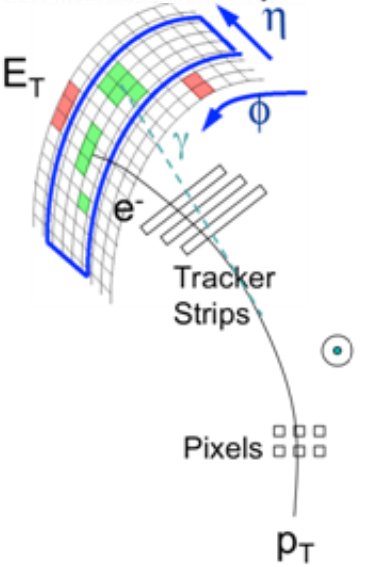
\includegraphics[width=0.75\textwidth]{figures/electronTrackAndSupercluster.png}
	\caption{The trajectory of a typical electron through the tracker and the ECAL.}
	\label{fig:eleTrackAndSC}
\end{figure}

Following reconstruction, the energies of electrons were corrected using $Z \rightarrow ee$ decays.  $Z \rightarrow ee$ 
events in data and simulations were compared, and two differences were found.  The dilepton mass distribution in simulated 
events was narrower, indicating better energy resolution, and the peak (in $\GeV$) was higher, indicating a higher 
energy scale.  Both the energy resolution and scale affect the efficiency of electron $\Et$ requirements, so the 
energies of electrons in data and simulated events were corrected such that the $Z \rightarrow ee$ dilepton mass peak 
positions and widths were identical.


\section{Jet Reconstruction}
\label{sec:jetReco}
%RESUME HERE

Through hadronization, photon radiation, and leptonic weak decays, quarks produced jets of photons, hadrons, and leptons.  Jet 
reconstruction began by reconstructing photons, electrons and muons, and charged and neutral hadrons.  Each charged hadron was 
reconstructed in a similar way to electrons, by geometrically matching an energy measured in an HCAL tower to a reconstructed 
track.  A charged hadron could also contain an ECAL SC if the SC $(\eta, \phi)$ position matched the HCAL tower.  Each neutral 
hadron was reconstructed as an HCAL tower, possibly associated with an ECAL SC, whose $(\eta, \phi)$ position did not match any 
reconstructed track.  Similarly, each photon was reconstructed as an ECAL SC whose position did not match any reconstructed track.  
After reconstructing individual particles, jets were reconstructed as clusters of individual particles, as shown in Figure 
\ref{fig:jetClustering}.

\begin{figure}[h]
	\centering
	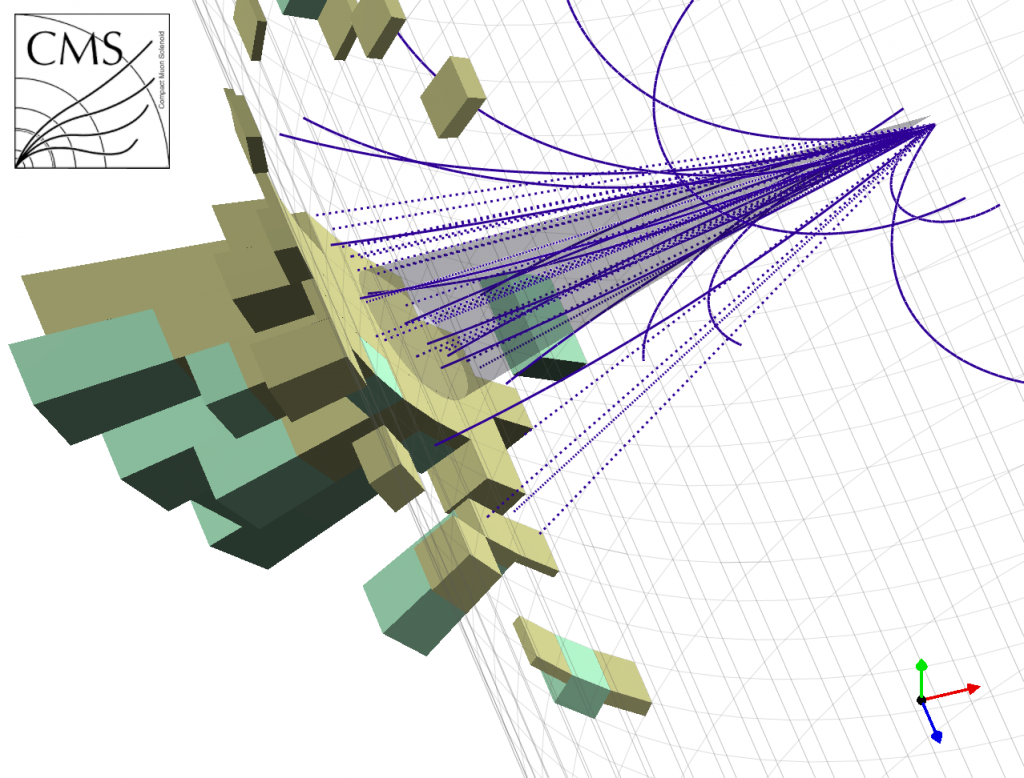
\includegraphics[width=0.75\textwidth]{figures/jetClusteringInCMS.png}
	\caption{A cone of reconstructed particles clustered into a jet, with the reconstructed vertex on the right.  
	From the CMS Experiment.}
	\label{fig:jetClustering}
\end{figure}

In each collision event, every reconstructed particle was considered a jet candidate, except charged hadrons that did not come 
from the reconstructed vertex with the highest $\sum \pt$.  Using the anti-$k_{T}$ algorithm \cite{antikt}, reconstructed particles 
were clustered into jets, each approximately $\Delta R = 0.4$ wide, based on their individual energies and trajectories.  Each jet's 
energy was the total energies of all constituents, and its $(\eta, \phi)$ trajectory was the energy-weighted average trajectory of 
all its constituents.


\section{Conclusion}
\label{sec:recoConclusion}
Energetic electrons, muons and jets produced in collisions were reconstructed using several CMS sub-detectors and high energy 
reconstruction algorithms.  Additional selections were applied to reconstructed leptons and jets to increase sensitivity to the \WR 
signal relative to ST processes that produced $\ell\ell jj$ events.

%%%%%%%%%%%%%%%%%%%%%%%%%%%%%%%%%%%%%%%%%%%%%%%%%%%%%%%%%%%%%%%%%%%%%%%%%%%%%%%%
